\documentclass[10pt,a4paper]{article}

\usepackage[utf8]{inputenc}
\usepackage[polish]{babel}
\usepackage[T1]{fontenc}
\usepackage{makecell}
\usepackage{indentfirst}
\usepackage{graphicx}
\usepackage{placeins}

\usepackage{tocloft}
\renewcommand{\cftsecleader}{\cftdotfill{\cftdotsep}}
\usepackage[hidelinks]{hyperref}

\usepackage[explicit]{titlesec}
\titleformat{\section}{\bfseries\large}{\thesection.}{0.5em}{#1}
\titleformat{\subsection}{\bfseries}{\thesubsection.}{0.5em}{#1}

\newcommand{\quotes}[1]{``#1''}

\title{Techniki internetowe \\ \large Dokumentacja wstępna projektu \quotes{TinDox}}
\author{
    \begin{tabular}{p{6em}p{6em}p{6em}p{6em}}
        \makecell{Jakub \\ Mazurkiewicz} &
        \makecell{Damian \\ Piotrowski} &
        \makecell{Anna \\ Pyrka} &
        \makecell{Łukasz \\ Reszka}
    \end{tabular}
}
\date{Semestr 21Z}

\begin{document}
\maketitle
\tableofcontents
\pagebreak

\section{Cel projektu}
Celem projektu jest opracowanie protokołu do wymiany plików przez sieć IPv4. Zakłada się także stworzenie wydajnego serwera oraz klientów na wybrane platformy.

\section{Protokół TDP}

\subsection{Opis}
TDP to protokół komunikacyjny typu serwer--klient wykorzystujący protokół sterowania transmisją (\href{https://en.wikipedia.org/wiki/Transmission_Control_Protocol}{TCP}). Umożliwia dwukierunkowy transfer plików oraz przeglądanie katalogów znajdujących się na zdalnym dysku.

\begin{figure}[ht]
\centering
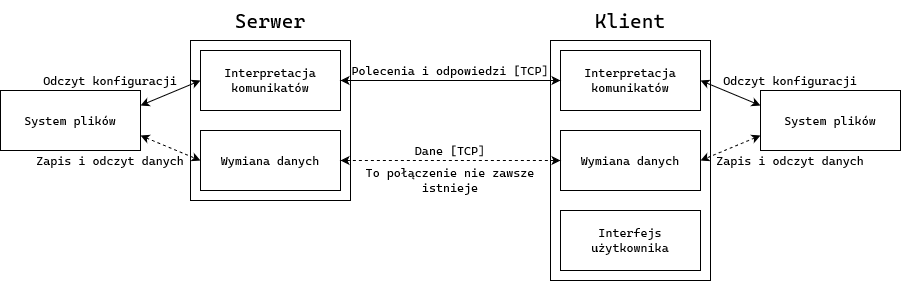
\includegraphics[width=1.001\textwidth]{img/session.png}
\caption{\label{fig:session.png}Schemat sesji inspirowany protokołem FTP.}
\end{figure}
\FloatBarrier

Komunikaty w protokole wymieniane są za pośrednictwem połączenia głównego (na rysunku oznaczonym jako \quotes{Polecenia i odpowiedzi}). Dane są przesyłane za pośrednictwem dodatkowego połączenia TCP (na rysunku oznaczonym jako \quotes{Dane}) tworzonego tylko na potrzeby pobierania i ładowania plików. Po zakończeniu jednej z tych operacji połączenie nie jest od razu zamykane -- może zostać użyte do kolejnych transferów.

\subsection{Słownik pojęć}
\begin{enumerate}
    \item TDP -- TinDox Protocol.
    \item Aktualny katalog -- każdy zalogowany użytkownik posiada przypisany do siebie katalog bieżący, czyli ten, w którym się aktualnie znajduje.
    \item Sól -- krótki, losowo wygenerowany ciąg składający się z wielkich i małych liter alfabetu łacińskiego oraz cyfr, identyfikujący pewną operację lub plik.
    \item Kod operacji -- losowo wygenerowany 32-bitowy kod identyfikujący pewną złożoną operację (np. pobieranie pliku).
\end{enumerate}

\pagebreak
\subsection{Metoda autoryzacji}
\begin{figure}[ht]
\centering
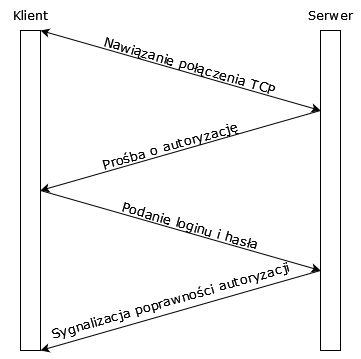
\includegraphics[width=0.6\textwidth]{img/auth.png}
\caption{\label{fig:auth.png}Schemat autoryzacji}
\end{figure}
\FloatBarrier
W przypadku niepomyślnej autoryzacji serwer wysyła do klienta ponowną prośbę o podanie danych. Po trzech nieudanych próbach serwer zamyka połączenie.

\subsection{Poruszanie się po katalogach}
Klient ma możliwość przejścia do katalogu domowego lub o jeden poziom względem bieżącego katalogu. Analogicznym działaniem w systemie Linux jest instrukcja \texttt{cd}.

\subsection{Wyświetlanie aktualnego katalogu}
Klient ma możliwość wyświetlenia ścieżki do aktualnego katalogu. Analogicznym działaniem w systemie Linux jest instrukcja \texttt{pwd}.

\subsection{Wypisywanie katalogów}
\noindent Istnieją dwie możliwości:
\begin{enumerate}
    \item Można wypisać wszystkie katalogi zaczynając od katalogu domowego (analogiczne polecenie systemowe to \texttt{tree}),
    \item Można wypisać podkatalogi i pliku znajdujące się w bieżącym katalogu (analogiczne polecenie systemowe \texttt{ls}).
\end{enumerate}

\subsection{Tworzenie katalogów}
Możliwe jest tworzenie katalogów tylko wewnątrz bieżącego katalogu, pojedynczo. Jeśli katalog o podanej nazwie już istnieje użytkownik otrzyma błąd.

Od momentu podania nazwy nowego katalogu jest ona już \quotes{zajęta}, w przypadku gdy dwie osoby spróbują stworzyć w tym samym czasie katalog o tej samej nazwie, jedna z nich otrzyma błąd.

\subsection{Tworzenie plików}
\begin{itemize}
    \item Scenariusz główny:
    \begin{enumerate}
        \item Klient wysyła do serwera żądanie utworzenia pliku o wskazanej nazwie w folderze, w którym obecnie się znajduje,
        \item Serwer sprawdza, czy w danym katalogu istnieje już plik o danej nazwie,
        \item Serwer tworzy plik o podanej nazwie w odpowiednim katalogu,
        \item Serwer wysyła do klienta potwierdzenie utworzenia nowego pliku.
    \end{enumerate}

    \item Scenariusz alternatywny -- próba utworzenia w \quotes{folderze klienta} pliku o tej samej nazwie co inny plik:
    \begin{enumerate}
        \item Kroki 1 -- 2 scenariusza głównego,
        \item Serwer wysyła do klienta odmowę wykonania operacji.
    \end{enumerate}
\end{itemize}

\subsection{Usuwanie plików i katalogów}
\begin{itemize}
    \item Scenariusz główny:
    \begin{enumerate}
        \item Klient wysyła do serwera żądanie usunięcia wskazanego pliku lub katalogu,
        \item Serwer sprawdza, czy istnieje katalog (lub plik) do usunięcia,
        \item Serwer sprawdza, czy w katalogu do usunięcia ktoś się znajduje lub czy plik do usunięcia jest aktualnie pobierany,
        \item Jeśli nie, to serwer usuwa katalog (lub plik) i wysyła potwierdzenie usunięcia do klienta.
    \end{enumerate}

    \item Scenariusz alternatywny I -- w katalogu do usunięcia ktoś się znajduje lub plik do usunięcia jest pobierany:
    \begin{enumerate}
        \item Kroki 1 -- 3 scenariusza głównego,
        \item Serwer wysyła do klienta odmowę wykonania operacji.
    \end{enumerate}

    \item Scenariusz alternatywny II -- próba usunięcia nieistniejącego pliku lub katalogu:
    \begin{enumerate}
        \item Kroki 1 -- 2 scenariusza głównego,
        \item Serwer wysyła do klienta odmowę wykonania operacji.
    \end{enumerate}
\end{itemize}

\subsection{Zmienianie nazwy plików i katalogów}
\begin{itemize}
    \item Scenariusz główny:
    \begin{enumerate}
        \item Klient wysyła do serwera żądanie zmiany nazwy pliku lub katalogu,
        \item Serwer sprawdza, czy istnieje plik lub katalog o tej samej nazwie w danym katalogu,
        \item Jeśli jest to plik, serwer sprawdza, czy jest on aktualnie pobierany,
        \item Jeśli jest to katalog, serwer sprawdza, czy aktualnie ktoś się w nim znajduje,
        \item Jeśli nie, serwer zmienia nazwę danego pliku lub katalogu i wysyła potwierdzenie do klienta.
    \end{enumerate}

    \item Scenariusz alternatywny I -- istnieje już plik lub katalog o tej samej nazwie:
    \begin{enumerate}
        \item Kroki 1 -- 2 scenariusza głównego,
        \item Serwer wysyła do klienta odmowę zmiany nazwy.
    \end{enumerate}

    \item Scenariusz alternatywny II -- próba zmiany nazwy pliku który jest obecnie pobierany:
    \begin{enumerate}
        \item Kroki 1 -- 3 scenariusza głównego,
        \item Serwer wysyła do klienta odmowę zmiany nazwy.
    \end{enumerate}

    \item Scenariusz alternatywny III -- próba zmiany nazwy katalogu w którym ktoś się znajduje:
    \begin{enumerate}
        \item Kroki 1 -- 4 scenariusza głównego,
        \item Serwer wysyła do klienta odmowę zmiany nazwy.
    \end{enumerate}
\end{itemize}

\subsection{Kopiowanie lub przenoszenie plików między katalogami}
\begin{itemize}
    \item Scenariusz główny:
    \begin{enumerate}
        \item Klient wysyła do serwera żądanie skopiowania pliku o danej nazwie do zadanego katalogu,
        \item Serwer sprawdza, czy istnieje katalog, do którego chcemy skopiować plik,
        \item Serwer sprawdza, czy w danym katalogu istnieje już plik o danej nazwie,
        \item Jeśli nie, serwer kopiuje plik do podanego katalogu.
    \end{enumerate}

    \item Scenariusz alternatywny I -- plik który chcemy skopiować jest w katalogu, w którym obecnie się nie znajdujemy:
    \begin{enumerate}
        \item Kroki 1  scenariusza głównego,
        \item Serwer wysyła do klienta odmowę skopiowania pliku.
    \end{enumerate}


    \item Scenariusz alternatywny II -- próba skopiowania pliku do katalogu, który nie istnieje:
    \begin{enumerate}
        \item Kroki 1 -- 2 scenariusza głównego,
        \item Serwer tworzy katalog o podanej nazwie, a następnie kopiuje do niego plik.
    \end{enumerate}

    \item Scenariusz alternatywny III -- próba skopiowania pliku w miejsce gdzie istnieje już inny o tej samej nazwie:
    \begin{enumerate}
        \item Kroki 1 -- 3 scenariusza głównego,
        \item Serwer wysyła do klienta odmowę skopiowania pliku.
    \end{enumerate}
\end{itemize}

\subsection{Pobieranie plików}
\noindent Klient może pobrać dany plik z serwera z aktualnego katalogu pod warunkiem, że ma do tego odpowiednie uprawnienia:
\begin{itemize}
    \item Scenariusz główny:
    \begin{enumerate}
        \item Klient wysyła pytanie o zgodę na pobranie pliku. Zawiera się w niej przede wszystkim nazwa przesyłanego pliku,
        \item Serwer, po zweryfikowaniu uprawnień użytkownika, wysyła zgodę na pobieranie wraz z dodatkowymi informacjami (np. rozmiar pliku, jaki jest największy możliwy pakiet do odebrania, kod identyfikujący operację),
        \item Klient nawiązuje dodatkowe połączenie TCP z serwerem, które będzie wykorzystywane do przesyłania danych,
        \item Serwer dzieli plik na małe pakiety i wysyła je do klienta,
        \item Klient odbiera fragmenty od serwera i dopisuje je do pliku o nazwie \quotes{\texttt{[NAZWA-ŁADOWANEGO-PLIKU].[SÓL].partial}} reprezentującego częściowo pobrane dane.
        \item Ostatnim pakietem wysłanym przez serwer jest informacja o zakończeniu ładowania,
        \item Aplikacja klienta zmienia nazwę pliku częściowego na docelową,
        \item Utworzone wcześniej dodatkowe połączenie TCP nie jest zamykane od razu -- istnieje możliwość wykorzystania go do kolejnych pobrań (lub ładowań).
    \end{enumerate}

    \item Scenariusz alternatywny I - odmowa pobierania:
    \begin{enumerate}
        \item Krok 1 scenariusza głównego,
        \item Klient otrzymuje odmowę pobierania pliku -- użytkownik dostaje informację o niepowodzeniu operacji.
    \end{enumerate}

    \item Scenariusz alternatywny II -- dodatkowe połączenie TCP z serwerem zostało wcześniej zestawione:
    \begin{enumerate}
        \item Kroki 1 -- 2 scenariusza głównego,
        \item Dodatkowe połączenie już istnieje -- serwer i klient będą je wykorzystywać do przesyłania danych,
        \item Kroki 4 -- 8 scenariusza głównego.
    \end{enumerate}

    \item Scenariusz alternatywny III -- dodatkowe połączenie TCP nie mogło zostać zestawione:
    \begin{enumerate}
        \item Kroki 1 -- 2 scenariusza głównego,
        \item Dodatkowe połączenie nie mogło zostać zestawione -- użytkownik dostaje informację o niepowodzeniu operacji.
    \end{enumerate}

    \item \textbf{Scenariusz alternatywny IV -- przerwanie połączenia z siecią w trakcie pobierania pliku}:
    \begin{enumerate}
        \item Kroki 1 -- 4 scenariusza głównego,
        \item Przerwanie połączenia ze strony klienta lub serwera,
        \item Serwer zapisuje do specjalnego pliku informację o przerwanej operacji. Zawiera się w niej między innymi nazwa użytkownika pobierającego plik, kod operacji oraz ostatni wysłany fragment pliku,
        \item W tym samym czasie klient zapisuje do pliku informację o przerwanej operacji. Zawiera się w niej między innymi lokalizacja pliku \texttt{.partial} i kod operacji,
        \item Klient i serwer oczekują na odzyskanie łączności z siecią,
        \item Klient nawiązuje ponownie połączenie z serwerem, loguje się na swoje konto,
        \item Klient sprawdza czy żadna operacja nie została wcześniej przerwana. Tak jest, zatem kieruje do użytkownika zapytanie o ponowienie operacji,
        \item Dwa możliwe scenariusze:
        \begin{itemize}
            \item Użytkownik ponawia pobieranie pliku:
            \begin{enumerate}
                \item Aplikacja klienta wysyła prośbę o ponowienie operacji pobierania,
                \item Serwer, po zweryfikowaniu że taka operacja faktycznie miała wcześniej miejsce, wyraża zgodę na ponowienie,
                \item Kroki 3 -- 8 scenariusza głównego.
            \end{enumerate}

            \item Użytkownik kończy operację pobierania pliku:
            \begin{enumerate}
                \item Aplikacja klienta wysyła informację o tym, że pobieranie nie będzie ponawiane,
                \item Serwer po otrzymaniu informacji usuwa wpis utworzony w punkcie 3 scenariusza alternatywnego IV.
            \end{enumerate}
        \end{itemize}
    \end{enumerate}
\end{itemize}

\subsection{Ładowanie plików}
\noindent Klient może załadować plik na serwer do aktualnego katalogu:
\begin{itemize}
    \item Scenariusz główny:
    \begin{enumerate}
        \item Klient wysyła pytanie o zgodę na załadowanie pliku. Zawiera się w niej między innymi nazwa przesyłanego pliku oraz jego rozmiar,
        \item Serwer, po zweryfikowaniu uprawnień użytkownika, wydaje zgodę na ładowanie wraz z dodatkowymi informacjami (np. jaki jest maksymalny możliwy rodzaj pojedynczego pakietu, kod identyfikujący operację),
        \item Klient nawiązuje dodatkowe połączenie TCP z serwerem, które będzie wykorzystywane do przesyłania danych,
        \item Klient dzieli plik na małe pakiety i wysyła je do serwera,
        \item Serwer odbiera fragmenty od klienta i dopisuje je do pliku o nazwie \quotes{\texttt{[NAZWA-ŁADOWANEGO-PLIKU].[SÓL].partial}} reprezentującego częściowo załadowane dane. Plik ten nie jest wyświetlany w przypadku żądania wypisania katalogu przez klienta,
        \item Ostatnim pakietem wysłanym przez klienta jest informacja o zakończeniu ładowania,
        \item Serwer zmienia nazwę pliku częściowego na docelową,
        \item Utworzone wcześniej dodatkowe połączenie TCP nie jest zamykane od razu -- istnieje możliwość wykorzystania go do kolejnych ładowań (lub pobrań).
    \end{enumerate}

    \item Scenariusz alternatywny I - odmowa ładowania:
    \begin{enumerate}
        \item Krok 1 scenariusza głównego,
        \item Klient otrzymuje odmowę ładowania pliku -- użytkownik dostaje informację o niepowodzeniu operacji.
    \end{enumerate}

    \item Scenariusz alternatywny II -- dodatkowe połączenie TCP z serwerem zostało wcześniej zestawione:
    \begin{enumerate}
        \item Kroki 1 -- 2 scenariusza głównego,
        \item Dodatkowe połączenie już istnieje -- serwer i klient będą je wykorzystywać do przesyłania danych,
        \item Kroki 4 -- 8 scenariusza głównego.
    \end{enumerate}

    \item Scenariusz alternatywny III -- dodatkowe połączenie TCP nie mogło zostać zestawione:
    \begin{enumerate}
        \item Kroki 1 -- 2 scenariusza głównego,
        \item Dodatkowe połączenie nie mogło zostać zestawione -- użytkownik dostaje informację o niepowodzeniu operacji.
    \end{enumerate}

    \item Scenariusz alternatywny IV -- klient wysłał nieprawidłowy fragment pliku:
    \begin{enumerate}
        \item Kroki 1 -- 4 scenariusza głównego,
        \item Klient wysłał nieprawidłowy fragment pliku -- serwer wysyła informację o błędzie i kończy operację. Nie zamyka on jednak zestawionego połączenia TCP -- może być wykorzystane później.
    \end{enumerate}

    \item \textbf{Scenariusz alternatywny V -- przerwanie połączenia z siecią w trakcie ładowania pliku}:
    \begin{enumerate}
        \item Kroki 1 -- 4 scenariusza głównego,
        \item Przerwanie połączenia ze strony klienta lub serwera,
        \item Serwer zapisuje do specjalnego pliku informację o przerwanej operacji. Zawiera się w niej między innymi nazwa użytkownika ładującego plik, kod operacji oraz ostatni odebrany fragment pliku,
        \item W tym samym czasie klient zapisuje do pliku informację o ostatnim wysłanym fragmencie pliku oraz lokalnej ścieżce do pliku,
        \item Klient i serwer oczekują na odzyskanie łączności z siecią,
        \item Klient nawiązuje ponownie połączenie z serwerem, loguje się na swoje konto,
        \item Klient sprawdza czy żadna operacja nie została wcześniej przerwana. Tak jest, zatem kieruje do użytkownika zapytanie o ponowienie operacji,
        \item Dwa możliwe scenariusze:
        \begin{itemize}
            \item Użytkownik ponawia ładowanie pliku:
            \begin{enumerate}
                \item Aplikacja klienta wysyła prośbę o ponowienie operacji ładowania,
                \item Serwer, po zweryfikowaniu że taka operacja faktycznie miała wcześniej miejsce, wyraża zgodę na ponowienie,
                \item Kroki 3 -- 8 scenariusza głównego.
            \end{enumerate}

            \item Użytkownik kończy operację ładowania pliku:
            \begin{enumerate}
                \item Aplikacja klienta wysyła informację o tym, że ładowanie nie będzie ponawiane,
                \item Serwer po otrzymaniu informacji usuwa wpis utworzony w punkcie 3 scenariusza alternatywnego V.
            \end{enumerate}
        \end{itemize}
    \end{enumerate}
\end{itemize}

\subsection{Struktura komunikatów}

\subsubsection{Polecenia dla serwera}
Polecenia w protokole TDP wysyłane są tekstowo, podobnie jak np. w protokole HTTP. W pierwszej linii komunikatu znajduje nazwa polecenia, natomiast w kolejnych jego parametry.

Poniższa tabela przedstawia nazwy poleceń w protokole TDP:
\begin{center}
    \begin{tabular}{l|l|l}
        \textbf{Polecenie} & \textbf{Opis} & \textbf{Parametry} \\
        \hline
        \texttt{auth} & Autoryzacja & Login i hasło \\
        \hline
        \texttt{cd} & Zmiana katalogu & Ścieżka do zmiany \\
        \hline
        \texttt{pwd} & Wyświetlanie aktualnego katalogu & --- \\
        \hline
        \texttt{ls} & Wypisywanie katalogów & \makecell[lt]{Parametry określające prośbę\\o zwrot dodatkowych informacji} \\
        \hline
        \texttt{tree} & Wypisywanie drzewa katalogów & --- \\
        \hline
        \texttt{mkdi} & Tworzenie katalogu & Nazwa nowego katalogu \\
        \hline
        \texttt{rm} & Usuwanie pliku lub katalogu & Nazwa pliku lub katalogu \\
        \hline
        \texttt{rname} & Zmiana nazwy pliku lub katalogu & Nazwa pliku oraz nowa nazwa \\
        \hline
        \texttt{cp} & Kopiowanie pliku lub katalogu & Nazwa pliku oraz miejsce docelowe \\
        \hline
        \texttt{mv} & Przenoszenie pliku lub katalogu & Nazwa pliku oraz miejsce docelowe \\
        \hline
        \texttt{dl} & Inicjacja pobierania & Nazwa pliku \\
        \hline
        \texttt{ul} & Inicjacja ładowania & Nazwa pliku oraz jego rozmiar \\
    \end{tabular}
\end{center}

\subsubsection{Odpowiedzi serwera na polecenia}
\noindent W odpowiedzi serwera w kolejnych liniach zawierają się następujące informacje:
\begin{enumerate}
    \item Kod zwrotny -- określa np. status powodzenia operacji, informację o ewentualnym błędzie,
    \item Nazwa polecenia -- nazwa polecenia wykonanego przez użytkownika,
    \item Szczegóły odpowiedzi -- rezultat wykonanego polecenia. Przykładowo, dla polecenia \texttt{ls} w odpowiedzi w kolejnych liniach zawarte będą nazwy plików i katalogów wraz z np. datami ich utworzenia.
\end{enumerate}

\subsubsection{Transmisja danych}
Przy pobieraniu lub ładowaniu plików na serwer dane przesyłane są w małych pakietach w sposób binarny. Poniższy rysunek przedstawia strukturę takiego binarnego pakietu:

\begin{figure}[ht]
\centering
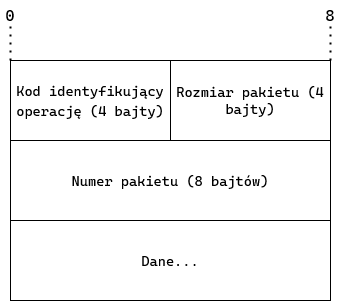
\includegraphics[width=0.6\textwidth]{img/packet.png}
\caption{\label{fig:packet.png}Pakiet używany przy pobieraniu lub ładowaniu}
\end{figure}
\FloatBarrier

\pagebreak
\section{Serwer}

\subsection{Słownik pojęć}
\noindent Pojęcia używane w tej sekcji:
\begin{enumerate}
    \item TDS -- TinDox Server.
    \item Instancja serwera -- katalog zawierający katalog podrzędny o nazwie \texttt{.tds}, w którym znajdują pliki konfiguracyjne potrzebne do uruchomienia serwera. Instancja jest również korzeniem systemu plików widocznego przez klienta.
    \item IO - wejście i wyjście.
\end{enumerate}

\subsection{Wymagania funkcjonalne}

\begin{enumerate}
    \item Możliwość szybkiego utworzenia instancji serwera w dowolnym miejscu na dysku.
    \item Tworzenie, modyfikacja i usuwanie użytkowników uprawnionych do korzystania z dysku sieciowego.
    \item Realizacja komunikacji z klientami z wykorzystaniem gniazd BSD.
    \item Wydajne IO dzięki wykorzystaniu zasobów systemowych:
    \begin{itemize}
        \item Wykorzystanie efektywnej liczby wątków do obsługi wielu klientów jednocześnie,
        \item Wykorzystanie linuksowego mechanizmu \texttt{epoll} do sprawnej obsługi aktywnych klientów.
    \end{itemize}
    \item Bezbłędne zamykanie połączeń z klientami oraz całego serwera.
    \item Prawidłowe reagowanie na sygnały systemowe (np. użycie \texttt{Ctrl+C} w terminalu powinno prawidłowo zakończyć działanie serwera).
    \item Monitorowanie połączeń przychodzących oraz błędów serwera, tworzenie raportów i zarządzanie nimi.
\end{enumerate}

\subsection{Wymagania niefunkcjonalne}

\begin{enumerate}
    \item Konfigurowalność -- serwer będzie wykorzystywał plik konfiguracyjny w formacie TOML. Edytując go, użytkownik będzie mógł dostosować serwer do możliwości swojego komputera, co oznacza między innymi:
    \begin{itemize}
        \item Możliwość wyboru maksymalnej ilości wątków używanych przez serwer (domyślnie będzie to wartość zwracana przez funkcję z języka \texttt{C++} -- \texttt{std::thread::hardware\_concurrency()}),
        \item Możliwość wyboru maksymalnej ilości klientów w sesji.
    \end{itemize}

    \item Wydajność -- serwer powinien sprawnie obsługiwać wiele żądań jednocześnie przy wykorzystaniu optymalnej ilości zasobów systemu operacyjnego.

    \item Bezpieczeństwo -- serwer powinien być odporny na złośliwe zapytania. Oznacza to, że w aplikacji nie wystąpią podatności takie jak np. \href{https://en.wikipedia.org/wiki/Arbitrary_code_execution}{RCE}.
\end{enumerate}

\subsection{Polecenia linii komend}
\noindent Przykładowe polecenia linii komend udostępniane przez serwer:
\begin{itemize}
    \item \texttt{./tds init} -- tworzenie instancji serwera w bieżącym katalogu.
    \item \texttt{./tds run <flags>} -- uruchomienie instancji serwera w bieżącym katalogu.
    \item \texttt{./tds log <flags>} -- przeglądanie logów serwera.
    \item \texttt{./tds user <flags>} -- manipulacja listą użytkowników (np. dodawanie nowego użytkownika \quotes{\texttt{./tds user add ...}}).
    \item \texttt{./tds config <flags>} -- zmiana wartości parametrów serwera.
\end{itemize}

\subsection{Narzędzia i biblioteki}

\bgroup
    \begin{center}
        \def\arraystretch{1.3}
        \begin{tabular}{c|c|c}
            \textbf{Element} & \textbf{Narzędzia} & \textbf{Wersja} \\
            \hline
            Język programowania & \texttt{C++} & ISO/IEC 14882:2020 \\
            \hline
            Kompilator & \makecell{\texttt{g++} \\ \texttt{clang}} & \makecell{11.1.0 \\ 13.0.0} \\
            \hline
            System budowania & \texttt{\href{https://cmake.org/}{CMake}} & \makecell{3.18.4} \\
            \hline
            Automatyzacja testów & \texttt{CTest} & \makecell{3.18.4} \\
            \hline
            Testy jednostkowe & \texttt{Catch2} & 3.0.0 \\
            \hline
            Obsługa formatu TOML & \texttt{\href{https://github.com/marzer/tomlplusplus}{@marzer/tomlplusplus}} & 2.5.0 \\
            \hline
            Platforma docelowa & \texttt{Linux x86-64} & 4.0.0
        \end{tabular}
    \end{center}
\egroup

\section{Klient mobilny}

\subsection{Opis klienta}
Połączenie z serwerem za pomocą klienta w aplikacji mobilnej zaimplementowane z użyciem języka kotlin w środowisku Android Studio. Za ich pomocą powstanie prosta aplikacja mobilna z interakcyjnym interfejsem graficznym reprezentująca nasz zdalny system plików. Aplikacja będzie budowana na system Android.

\subsection{Narzędzia i biblioteki}
\bgroup
    \begin{center}
        \def\arraystretch{1.3}
        \begin{tabular}{c|c}
            \textbf{Element} & \textbf{Narzędzia} \\
            \hline
            Język programowania & \texttt{Kotlin} \\
            \hline
            Kompilator & \texttt{kotlinc} \\
            \hline
            IDE & \texttt{Android Studio} \\
            \hline
            Platforma docelowa & \texttt{Android}
        \end{tabular}
    \end{center}
\egroup

\section{Klient okienkowy}

\subsection{Opis klienta}
Połączenie z serwerem realizowane przez klienta okienkowego zaimplementowanego z użyciem języka Java i klasy Socket, która reprezentuje gniazda klienckie. Po uruchomieniu klient podejmie próbę połączenia z serwerem. W przypadku udanego połączenia aplikacja umożliwi interakcję ze zdalnym systemem plików.

\subsection{Narzędzia i biblioteki}
\bgroup
    \begin{center}
        \def\arraystretch{1.3}
        \begin{tabular}{c|c}
            \textbf{Element} & \textbf{  Narzędzia  } \\
            \hline
            Język programowania & \texttt{Java}  \\
            \hline
            Kompilator & \texttt{javac} \\
            \hline
            Testy jednostkowe & \texttt{JUnit}  \\
            \hline
            System budowania & \texttt{Gradle}  \\
        \end{tabular}
    \end{center}
\egroup

\section{Klient konsolowy}

\subsection{Opis klienta}
Połączenie z serwerem realizowane poprzez klienta zaimplementowanego przy użyciu biblioteki \texttt{ncurses} i języka \texttt{C}. Ncurses to zbiór funkcji i narzędzi pozwalających tworzyć zgrabne TUI. Wykorzystując elementy biblioteki powstanie narzędzie do wykonywania operacji plikowych na zdalnym systemie plików.

Klient konsolowy przeznaczony jest na system \texttt{Ubuntu}. Będzie kompilowany z wykorzystaniem \texttt{gcc} oraz budowany z wykorzystaniem \texttt{CMake}.

\subsection{Narzędzia i biblioteki}

\bgroup
    \begin{center}
        \def\arraystretch{1.3}
        \begin{tabular}{c|c|c}
            \textbf{Element} & \textbf{Narzędzia} & \textbf{Wersja} \\
            \hline
            Język programowania & \texttt{C} & ISO/IEC 9899:2011 \\
            \hline
            Kompilator & \makecell{\texttt{gcc}} & \makecell{10.3.0} \\
            \hline
            System budowania & \texttt{\href{https://cmake.org/}{CMake}} & \makecell{3.22.0} \\
            \hline
            TUI & \texttt{ncurses} & 6.2 \\
            \hline
            Platforma docelowa & \texttt{Linux x86-64} & 4.0.0
        \end{tabular}
    \end{center}
\egroup

\section{Metody testowania}

\begin{enumerate}
    \item Testy jednostkowe -- testowanie najważniejszych modułów poszczególnych projektów (np. modułu raportującego w serwerze lub składowych konstrukcji MVC w aplikacji mobilnej).
    \item Testy integracyjne -- testy weryfikujące poprawność komunikacji między największymi składnikami całego systemu (np. między klientem konsolowym a serwerem).
    \item \textit{Fuzzing} -- automatyczne testowanie reakcji serwera na losowe wiadomości przychodzące od klienta.
    \item Testy obciążeniowe -- zautomatyzowane testowanie wytrzymałości serwera na zapytania przychodzące od dużych ilości klientów.
    \item Testy penetracyjne -- testy wykonywane w celu znalezienia podatności w oprogramowaniu serwera oraz klientów.
    \item Testy empiryczne -- testy wykonywane w czasie prezentacji programów dowodzące poprawności ich działania.
\end{enumerate}

\section{Zespół}

\subsection{Środowisko deweloperskie}

\bgroup
    \begin{center}
        \def\arraystretch{1.3}
        \begin{tabular}{c|c|c}
            \textbf{Element} & \textbf{Narzędzia} & \textbf{Wersja} \\
            \hline
            System operacyjny & \texttt{\makecell{Ubuntu \\ Manjaro Linux \\ Windows \\ Arch Linux}} & \makecell{20.04, 21.10 \\ 21.1.6 \\ 10.0 \\ ---} \\
            \hline
            \makecell{Pomocniczy język \\ skryptowy\footnotemark[1]} & \texttt{\makecell{Python \\ Bash}} & \makecell{3.9.7 \\ 5.1.8} \\
            \hline
            Kontrola wersji & \texttt{git} & 2.32.0 \\
            \hline
            \makecell{Repozytorium \\ ITS\footnotemark[2] \\ Tablica kanban} & \texttt{\makecell{\href{https://github.com/JMazurkiewicz/TIN-project}{GitHub} \\ \href{https://github.com/JMazurkiewicz/TinDox/issues}{GitHub Issues} \\ \href{https://github.com/JMazurkiewicz/TinDox/projects/1}{GitHub Projects}}} & --- \\
            \hline
            CI/CD & \texttt{Github Actions} & --- \\
            \hline
            Dokumentacja & \texttt{\href{https://www.overleaf.com/read/knbjwfrmvhzq}{Overleaf}} & --- \\
        \end{tabular}
    \end{center}
\egroup
\footnotetext[1]{Języki skryptowe będą używane do np. symulowania złożonych przypadków testowych, automatyzacji testów.}
\footnotetext[2]{Issue tracking system.}

\subsection{Podział pracy}

\begin{center}
    \begin{tabular}{l|r}
        \textbf{Projekt} & \textbf{Wykonawca} \\
        \hline
        Serwer & Jakub Mazurkiewicz \\
        Klient mobilny & Damian Piotrowski \\
        Klient okienkowy & Anna Pyrka \\
        Klient konsolowy & Łukasz Reszka
    \end{tabular}
\end{center}

\end{document}
